% ============================================================================
% LA GÉOMÉTRIE DU SPECTRE DES NOMBRES PREMIERS
% Avec validations formelles Isabelle/HOL COMPLÈTES ET EXACTES
% Auteur : Philippe Thomas Savard
% Version française
% ============================================================================

\documentclass[a4paper,11pt]{article}

% ============================================================================
% PACKAGES
% ============================================================================
\usepackage[utf8]{inputenc}
\usepackage[T1]{fontenc}
\usepackage[french]{babel}
\usepackage{amsmath,amssymb,amsthm}
\usepackage{mathtools}
\usepackage{graphicx}
\graphicspath{{images/}{./images/}}
\usepackage{float}
\usepackage{booktabs}
\usepackage{array}
\usepackage{longtable}
\usepackage{multirow}
\usepackage{geometry}
\usepackage{fancyhdr}
\usepackage{titlesec}
\usepackage{tocloft}
\usepackage{xcolor}
\usepackage{listings}
\usepackage{listingsutf8}
\usepackage{tcolorbox}
\usepackage{enumitem}
\usepackage{caption}
\usepackage{hyperref} % hyperref doit être chargé en dernier

% ============================================================================
% CONFIGURATION DE LA PAGE
% ============================================================================
\geometry{margin=2.5cm}

% Configuration de la table des matières
\setcounter{tocdepth}{3}
\setcounter{secnumdepth}{3}

% Configuration des couleurs
\definecolor{holblue}{RGB}{0,102,153}
\definecolor{holgreen}{RGB}{0,128,0}
\definecolor{holpurple}{RGB}{102,0,153}
\definecolor{lightgray}{RGB}{245,245,245}
\definecolor{darkgray}{RGB}{50,50,50}

% Configuration des hyperliens
\hypersetup{
    colorlinks=true,
    linkcolor=holblue,
    urlcolor=holblue,
    citecolor=holblue
}

% ============================================================================
% CONFIGURATION LISTINGS POUR CODE HOL
% ============================================================================
\lstdefinelanguage{isabelle}{
  keywords={theory, imports, begin, end, definition, where, fun, lemma, theorem, proof, qed, shows, assumes, fixes, and, if, then, else, let, in, axiomatization, section, subsection, text},
  keywordstyle=\color{holblue}\bfseries,
  sensitive=true,
  morecomment=[l]{--},
  morecomment=[s]{(*}{*)},
  commentstyle=\color{holgreen}\itshape,
  stringstyle=\color{holpurple},
  morestring=[b]",
  literate=
           {λ}{{$\lambda$}}1 
           {→}{{$\rightarrow$}}1 
           {⟶}{{$\longrightarrow$}}1
           {⟹}{{$\Longrightarrow$}}1 
           {↔}{{$\leftrightarrow$}}1
           {∧}{{$\wedge$}}1 
           {∨}{{$\vee$}}1 
           {¬}{{$\neg$}}1
           {≤}{{$\leq$}}1 
           {≥}{{$\geq$}}1 
           {≠}{{$\neq$}}1
           {∈}{{$\in$}}1 
           {∀}{{$\forall$}}1 
           {∃}{{$\exists$}}1
           {⟷}{{$\longleftrightarrow$}}1
           {‹}{{$\langle$}}1 
           {›}{{$\rangle$}}1
           {⋀}{{$\bigwedge$}}1
           {⇒}{{$\Rightarrow$}}1
           {×}{{$\times$}}1
           {«}{{<<}}1
           {»}{{>>}}1
           {—}{{---}}1
           {é}{{\'e}}1 
           {è}{{\`e}}1 
           {ê}{{\^e}}1 
           {ë}{{\"e}}1
           {à}{{\`a}}1 
           {â}{{\^a}}1 
           {ä}{{\"a}}1
           {ù}{{\`u}}1 
           {û}{{\^u}}1 
           {ü}{{\"u}}1
           {ô}{{\^o}}1 
           {î}{{\^i}}1 
           {ï}{{\"i}}1
           {ç}{{\c{c}}}1
           {É}{{\'E}}1 
           {È}{{\`E}}1 
           {Ê}{{\^E}}1
           {À}{{\`A}}1 
           {Ô}{{\^O}}1
           {–}{{--}}1
           {'}{{`}}1
           {'}{{`}}1
           {"}{{``}}1
           {"}{{''}}1
}

\lstset{
  language=isabelle,
  basicstyle=\small\ttfamily,
  breaklines=true,
  breakatwhitespace=true,
  columns=flexible,
  keepspaces=true,
  showstringspaces=false,
  frame=none,
  backgroundcolor=\color{lightgray},
  xleftmargin=0.5cm,
  xrightmargin=0.5cm,
  inputencoding=utf8,
  extendedchars=true,
}

% ============================================================================
% ENVIRONNEMENTS PERSONNALISÉS
% ============================================================================
\tcbuselibrary{listings,skins,breakable}

\newtcolorbox{holcode}[1][]{
    enhanced,
    breakable,
    colback=lightgray,
    colframe=holblue,
    fonttitle=\bfseries,
    title={\textcolor{white}{Validation Isabelle/HOL}},
    coltitle=white,
    attach boxed title to top left={xshift=5mm,yshift=-2mm},
    boxed title style={colback=holblue},
    left=2mm,
    right=2mm,
    #1
}

\newenvironment{mydef}[1]{%
    \begin{tcolorbox}[colback=blue!5,colframe=holblue,title={\textbf{Définition : #1}}]
}{%
    \end{tcolorbox}
}

\newenvironment{exemple}[1][]{%
    \begin{tcolorbox}[colback=green!5,colframe=holgreen,title={\textbf{Exemple #1}}]
}{%
    \end{tcolorbox}
}

\newenvironment{resume}{%
    \begin{tcolorbox}[colback=purple!5,colframe=holpurple,title={\textbf{Résumé visuel}}]
}{%
    \end{tcolorbox}
}

% ============================================================================
% TITRE ET AUTEUR
% ============================================================================

\title{
    \vspace{-2cm}
    {\LARGE \textbf{La Géométrie du Spectre}}\\[0.5cm]
    {\LARGE \textbf{des Nombres Premiers}}\\[1cm]
    {\large Avec validations formelles Isabelle/HOL}\\[0.5cm]
    \rule{\textwidth}{0.4pt}
}

\author{
    \textbf{Philippe Thomas Savard}\\[0.3cm]
    \small Lévis, Chaudière-Appalaches, Québec, Canada\\
    \small 5354 rue du Menuet, Lévis, Québec, G6X 2Y6\\
    \small Téléphone : 418-487-8798
}

\date{
    \vspace{0.5cm}
    Date originale : 8 novembre 2025\\
    Révision : 18 janvier 2026\\
    Compilation HOL : Février 2026
}

% ============================================================================
% DÉBUT DU DOCUMENT
% ============================================================================
\begin{document}

\maketitle
\thispagestyle{empty}

\vspace{1cm}

\begin{abstract}
Ce document présente la \textbf{géométrie du spectre des nombres premiers}, une méthode originale développée par Philippe Thomas Savard pour étudier la distribution des nombres premiers. L'approche combine des suites fractionnaires, des rapports triangulaires et une analyse numérique métrique inspirée de la granulométrie. Toutes les démonstrations mathématiques sont accompagnées de leurs \textbf{validations formelles en Isabelle/HOL}, garantissant la rigueur logique des résultats présentés.
\end{abstract}

\newpage
\tableofcontents
\newpage

% ============================================================================
% SECTION 1 : INTRODUCTION
% ============================================================================
\section{Introduction et Déclaration de l'Auteur}

\subsection{Coordonnées de l'auteur}

\begin{center}
\begin{tabular}{ll}
\textbf{Lieu :} & Lévis, Chaudière-Appalaches \\
\textbf{Adresse :} & 5354 rue du Menuet, Lévis, Québec, Canada, G6X 2Y6 \\
\textbf{Téléphone :} & 418-487-8798 \\
\end{tabular}
\end{center}

\vspace{0.5cm}

Ce document a été rédigé sans financement, sans avantages matériels ou symboliques, et dans une totale liberté de conscience et de jugement. Ce texte est le fruit d'une expérience de pensée, illustrée par des calculs mathématiques, des schémas, des tableaux, ainsi que des exemples et explications. L'auteur n'est pas initié aux mathématiques au sens académique : il ne possède aucune formation spécialisée dans ce domaine. Il est ouvrier, et c'est en dehors des sentiers balisés qu'il a conçu ce document par pur plaisir intellectuel et en conséquence d'un intérêt profond pour les mathématiques.

\subsection{Un mot de l'auteur}

Le document que vous vous apprêtez à lire s'inscrit dans une quête quotidienne, intime et persistante, qui habite l'auteur depuis toujours. Une quête qui, probablement, ne le quittera jamais.

\begin{resume}
\textbf{Imaginez} un jeune élève fasciné par une propriété simple mais intrigante : entre deux nombres entiers consécutifs, il ne peut jamais y avoir moins qu'une unité. Cette observation élémentaire, enseignée dès l'école primaire, éveilla une profonde curiosité qui mena, des années plus tard, à la découverte présentée dans ce document.
\end{resume}

Très jeune, l'auteur s'intéressa à la distribution des nombres entiers. Il tenta une expérience naïve mais révélatrice : ajouter successivement la valeur de 1 unité à des nombres pairs. Par exemple :
\begin{itemize}
    \item $1 + 50 = 51$
    \item $1 + 100 = 101$
    \item $1 + 200 = 201$
    \item $1 + 800 = 801$
\end{itemize}

Il observa que les rapports entre ces ajouts donnaient tous $\frac{1}{2}$ :
\[
\frac{50}{100} = \frac{100}{200} = \frac{200}{400} = \frac{400}{800} = \frac{1}{2}
\]

\begin{resume}
\textbf{Visualisez} cette découverte comme une échelle où chaque barreau est exactement à mi-chemin entre le précédent et le suivant. Cette fraction constante $\frac{1}{2}$ apparaît comme un fil conducteur reliant tous les nombres entiers entre eux.
\end{resume}

Plus tard, au début du secondaire, l'auteur découvrit les nombres premiers. Un nombre premier est divisible uniquement par 1 et par lui-même. Les dix premiers nombres premiers sont : 2, 3, 5, 7, 11, 13, 17, 19, 23 et 29.

Ce souvenir resta enfoui pendant près de vingt ans, jusqu'en 2016. L'auteur reprit l'expérience avec les nombres premiers de 0 à 109, en excluant 2 et 5. Il constata que 66,66\% des nombres ainsi générés étaient premiers en effectuant +/- 50, 100, 200,
 400 et 800 a ces nombres. De plus en plus de ce nombre élevé de nombres premiers ainsi dévoilé. il avait tous entre eux 1/2 lorsque placés en relation.

C'est à cette époque qu'il commença à s'intéresser à l'hypothèse de Riemann et à se poser la question fondamentale :

\begin{center}
\fbox{\parbox{0.8\textwidth}{
\textbf{L'énigme de Bernhard Riemann :}\\
« Est-ce que tous les zéros non triviaux de la fonction zêta de Bernhard Riemann ont tous pour partie réelle $\frac{1}{2}$ ? »
}}
\end{center}

\subsection*{Sous-introduction philosophique}

\textbf{Question.} Comment la theorie ``L'Univers est au Carre'' pourrait-elle transformer notre comprehension philosophique de l'univers et quelles implications epistemologiques cela pourrait-il entrainer?

\medskip

\textbf{Reponse.} La theorie ``L'Univers est au Carre'', avec son approche geometrique originale, conduit a une reconceptualisation de la realite en reliant les mathematiques fondamentales a une comprehension 
plus universelle de l'ordre cosmique. Cette perspective pourrait influencer profondement notre vision philosophique en suggerant que l'univers peut etre compris comme une structure geometrique ordonnee, regie
 par des lois mathematiques precises et formalisees, notamment par le postulat unique de l'univers est au carre.

Sur le plan epistemologique, cette approche invite a reexaminer la nature meme de la connaissance: si l'univers est entierement rationnel et geometrique, la decouverte de ses lois devient une question de deduction¸
 et de formalisation plutot que d'observation empirique. Cela pourrait aussi impliquer une redefinition de la relation entre le connaissable et l'inobservable, en supposant que la complexite peut etre apprehendee par 
 des modeles mathematiques non conventionnels. L 


% ============================================================================
% SECTION 2 : PREMIÈRE PARTIE - GÉOMÉTRIE DU SPECTRE
% ============================================================================
\newpage
\section{Première Partie : La Géométrie du Spectre des Nombres Premiers}

\begin{figure}[H]
    \centering
    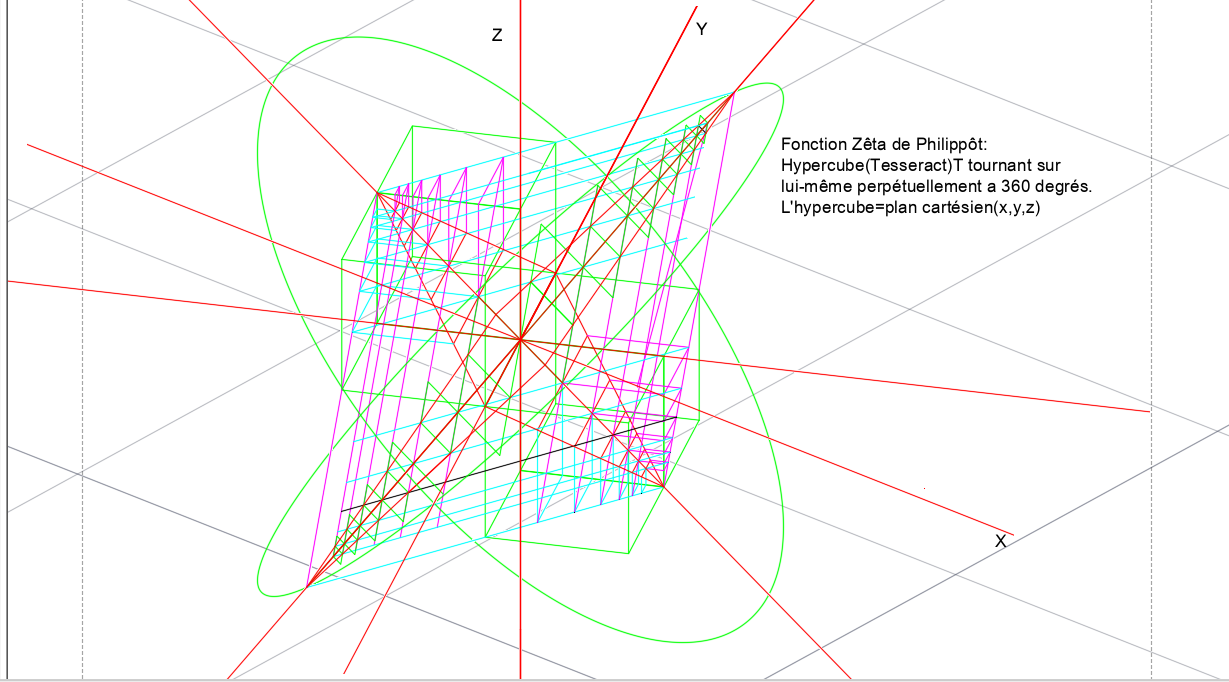
\includegraphics[width=0.9\textwidth]{fonction_zeta_riemann_philippot.png}
    \caption{Représentation de la fonction Zêta de Philippôt dans un plan $(x, y, z)$ -- L'hypercube (Tesseract) tourne sur lui-même perpétuellement à 360 degrés.}
    \label{fig:zeta}
\end{figure}

\begin{resume}
\textbf{Imaginez} un hypercube (tesseract) -- une figure géométrique à quatre dimensions -- tournant perpétuellement sur lui-même dans l'espace tridimensionnel. Cette rotation crée des projections dynamiques qui, selon l'auteur, encodent la distribution des nombres premiers.
\end{resume}

\subsection{Mouvement du plan cartésien et Tesseract}

En effet, le produit entre le périmètre d'un carré A et la mesure du diamètre d'un carré B est égal au produit du périmètre du carré B et de la mesure du diamètre du carré A. La figure de l'hypercube au repli type de la figure est démontré a l'aide de ce produit alternatif.
Le produit entre le diamètre du carré A par le périmètre du carré B égale au produit du diamètre du carré B par le périmètre du carré A, donne naissance a l'analyse numérique métrique qui sera détaillé dans ce document plus en profondeur. Deux produit alternatifs distincts
définissent le replient typique de l'hypercube? Le produit alternatif symétrique et le produit alternatif asymétrique. Les propriétée du produit alternatif assymétrique sont différentes de celui symétrique. Leproduit alternatif asymétrique pas du résultat du produit entre deux carrés,
mais bien le fruit du produit résultant de la déformation de l'hypercube formant un rectangle? Ce rectangle est divisé en sections. 4 sections différentes dont le produit des aires diagonalement opposé forme le produit alternatif. Ces aires comme le démontre l'exemple présenté dans le
document dont les valeur numérique des aires corespondre aux propriétés périmètres diamètres caractérisant le produit alternatif symétrique. Le résultat de ce produit alternatif asymétrique dont les aires opposé diagonalement possèdent les caractéristiques périmètres diamètres 
du produit alternatif symétrique. 

\begin{mydef}{Produit alternatif}
Ce produit alternatif à droite est, pour Savard, le résultat du mouvement du Tesseract. Deux carrés sont représentés :
\begin{itemize}
    \item Un carré de $1 \times 1$
    \item Un carré de $1.5 \times 1.5$
\end{itemize}
\end{mydef}

\begin{figure}[H]
    \centering
    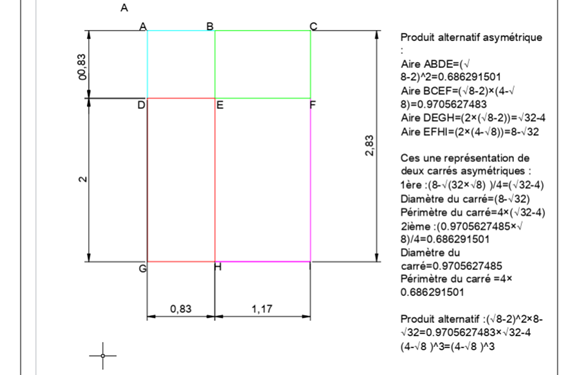
\includegraphics[width=0.85\textwidth]{asymetrique_alternatif_philippot.png}
    \caption{Analyse du mouvement de l'hypercube surface par surface -- Produit alternatif symétrique et asymétrique}
    \label{fig:hypercube}
\end{figure}


\subsection{Mouvement de l'hypercube surface par surface}


\subsubsection{Produit alternatif symétrique}

\begin{exemple}[: Calcul du produit alternatif symétrique]

\textbf{Carré A :}
\begin{itemize}
    \item Côté Carré A $= 1$
    \item Diamètre Carré A $= \sqrt{2}$
\end{itemize}

\textbf{Carré B :}
\begin{itemize}
    \item Côté Carré B $= 1.5$
    \item Diamètre Carré B $= \sqrt{4.5}$
\end{itemize}

\textbf{Produit alternatif à ajouter :}
\[
(1.5 \times 4) \times \sqrt{2} = \sqrt{4.5} \times 4
\]

\textbf{Résultat du produit :}
\[
\sqrt{72}
\]
\end{exemple}

\subsubsection{Produit alternatif asymétrique}

\begin{exemple}[: Calcul des aires -- Corrigé]
Les aires des différentes surfaces sont calculées comme suit :

\begin{align}
\text{Aire A} &= (\sqrt{8} - 2)^2 = 0.686291501 \\
\text{Aire B} &= 2 \times (4 - \sqrt{8}) \\
\text{Aire C} &= (\sqrt{8} - 2) \times (4 - \sqrt{8}) = 0.9705627485 \\
\text{Aire D} &= 2 \times (\sqrt{8} - 2) = \sqrt{32} - 4
\end{align}
\end{exemple}

\textbf{Transposition en relation périmètre-diamètre :}

Ce qui se transpose en :
\[
\text{Périmètre A} \times \text{Diamètre B} = \text{Diamètre A} \times \text{Périmètre B} \quad \text{(pour les aires)}
\]

\textbf{Produit alternatif corrigé :}
\[
0.9705627485 \times (\sqrt{32} - 4) = 0.686291501 \times 2 \times (4 - \sqrt{8})
\]

\textbf{Volume de l'hypercube :}
\[
(4 - \sqrt{8})^3 = (4 - \sqrt{8})^3 \quad \text{Volume de l'hypercube}
\]

\begin{resume}
Le résultat final pour le produit alternatif asymétrique révèle une valeur associable à un cube (puissance 3). Ce point permet d'associer le produit alternatif, à partir de surfaces de figures symétriques et asymétriques, au mouvement d'un tesseract en analysant son mouvement, une surface à la fois.
\end{resume}

% ============================================================================
% SECTION 3 : ANALYSE NUMÉRIQUE MÉTRIQUE
% ============================================================================
\newpage
\section{Analyse Numérique Métrique}

Cette section présente une analyse numérique métrique en lien avec la fonction Zêta de Philippôt.

\begin{figure}[H]
    \centering
    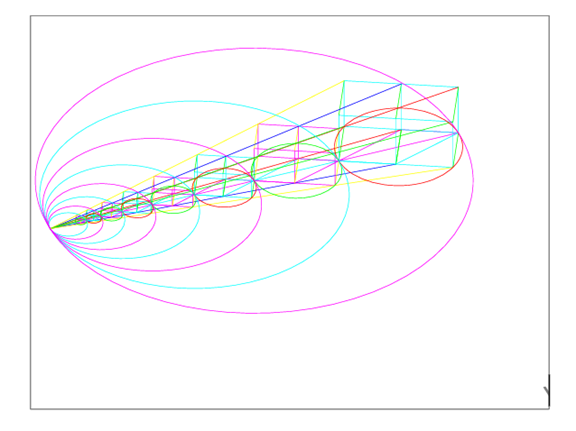
\includegraphics[width=0.9\textwidth]{analyse_numerique_metrique_cube.png}
    \caption{Représentation 3D de l'analyse numérique métrique -- Les cubes et pyramides internes}
    \label{fig:cube3d}
\end{figure}


\begin{resume}
L'analyse numerique metrique est une creation originale de l'auteur. Inspiree par un parallele avec l'analyse granulometrique pour demontre le raisonement. Cette approche constitue le fondement de sa methode : une transposition conceptuelle ou la structure des tamis devient un outil pour comprendre la distribution des grandeurs numeriques.

Visuellement, l'auteur -- Philippe Thomas Savard -- represente cette idee par une serie de parallelogrammes successifs. Une droite centrale traverse chacun d'eux, tandis que deux autres droites, tangentes aux sommets formes par les angles obtus, encadrent la figure. Dans une analyse granulometrique classique, chaque tamis impose une limite de passant correspondant a une taille de maille precise. La masse retenue sur chaque tamis doit respecter une valeur determinee, et l'ensemble des resultats peut etre represente sous forme de courbe ou de zone ombree definissant les limites acceptables.

Dans l'analyse numerique metrique, cette zone ombree correspond a l'espace compris entre les deux droites tangentes aux sommets obtus des parallelogrammes. Ces sommets representent, en alternance, la position de la suite A et de la suite B. Comme nous le verrons plus loin, le nombre de termes dans ces deux suites determine la position du nombre premier associe au rapport spectral 1/2. Cette alternance est analogue au produit alternatif ou le perimetre du carre A multiplie par le diametre du carre B est egal au diametre du carre A multiplie par le perimetre du carre B.

Chaque parallelogramme possede deux sommets obtus, et chacun de ces sommets correspond successivement a la position de la suite A ou de la suite B. Cette alternance structure l'ensemble de la progression.

Lorsqu'une analyse granulometrique est effectuee sur un sol de calibre 0 mm a 20 mm, la serie de tamis utilisee est simple : tous les tamis sont inferieurs ou egaux a 20 mm. En revanche, pour un sol de calibre 0 mm a 56 mm, deux types de sols sont presents : un premier de 0 mm a 20 mm, et un second jusqu'a 56 mm. Dans ce cas, une substitution doit etre effectuee dans la serie de tamis afin d'eviter que l'operateur n'ait l'impression que les granulats "remontent" les tamis. Il faut donc remplacer un tamis de la serie 0--20 mm par celui de la serie 0--56 mm situe immediatement au-dessus.

L'auteur note egalement une analogie interessante observee dans le systeme de numeration grecque : la lettre zeta vaut 7 bien qu'elle occupe la sixieme position, en raison de l'ancienne presence du digamma entre l'epsilon et le zeta (reference : Encyclopedie libre Wikipedia, lettre grecque Zeta). Cette observation souleve une question similaire pour les nombres premiers, qui appartiennent a l'ensemble des entiers mais se distinguent des nombres composes. Deux types de nombres entrent donc en jeu.

Pour aborder l'enigme de Riemann, l'auteur imagine un monticule de cailloux plus haut que lui-meme, ou chaque caillou -- meme les poussieres -- porte un nombre, de 0 a l'infini. L'echantillon representatif utilise est constitue des dix chiffres 0 a 9, qui permettent de composer tous les nombres possibles. Lors du prelevement, la circonference et la hauteur du monticule sont mesurees. Grace a la normalisation des tamis et a l'espacement constant entre eux, il devient alors possible de retrouver la position exacte de chaque caillou dans le monticule.

L'analyse numerique metrique transpose cette logique : une serie de parallelogrammes se succedent, chacun defini par deux petites diagonales opposees. Ces diagonales entretiennent entre elles un rapport constant de 1/2, de l'interieur vers l'exterieur. En trois dimensions, cette structure devient une serie de paires de cubes, formant un volume analogue a un tesseract -- un hypercube en deformation continue.
\end{resume}


\subsection{Analyse numérique métrique en 3 dimensions}

\begin{figure}[H]
    \centering
    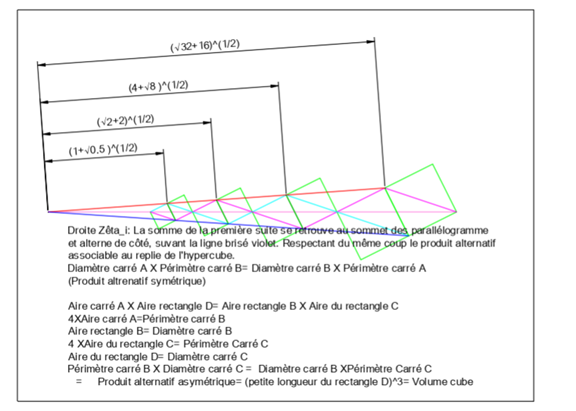
\includegraphics[width=0.85\textwidth]{analyse_numerique_metrique_haut.png}
    \caption{Vue de haut de l'analyse numérique métrique}
    \label{fig:anm_haut}
\end{figure}

\begin{figure}[H]
    \centering
    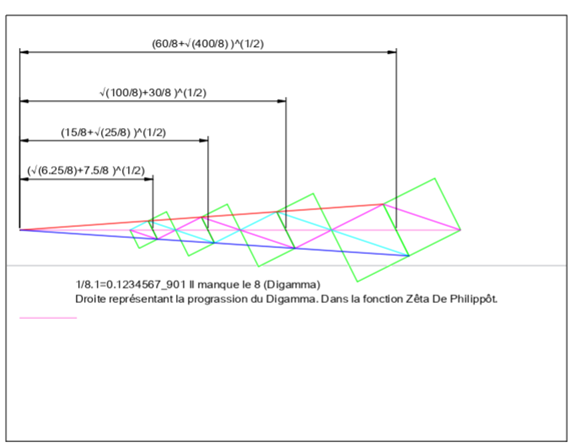
\includegraphics[width=0.85\textwidth]{analyse_numerique_metrique_centre.png}
    \caption{Analyse numérique métrique -- Vue centrale avec progression du Digamma}
    \label{fig:anm_centre}
\end{figure}

\begin{mydef}{Le Digamma}
Dans le système de numération grecque, le Zêta vaut 7, bien qu'il occupe la sixième position. Ceci est dû à l'ancienne existence du Digamma, situé entre l'Epsilon et le Zêta.

\textit{(Définition tirée de l'encyclopédie libre Wikipédia)}

Cette particularité -- une valeur qui ne correspond pas à la position -- rejoint l'idée de substitution évoquée dans l'analyse granulométrique qui comme pour la méthode lié au sol permet le tamisage d'un sol composé de deux granulat permet du a la substitution dans la suite B de comparer les nombres composés et les nombres premiers.
\end{mydef}

\subsection{Géométrie des suites}

\begin{figure}[H]
    \centering
    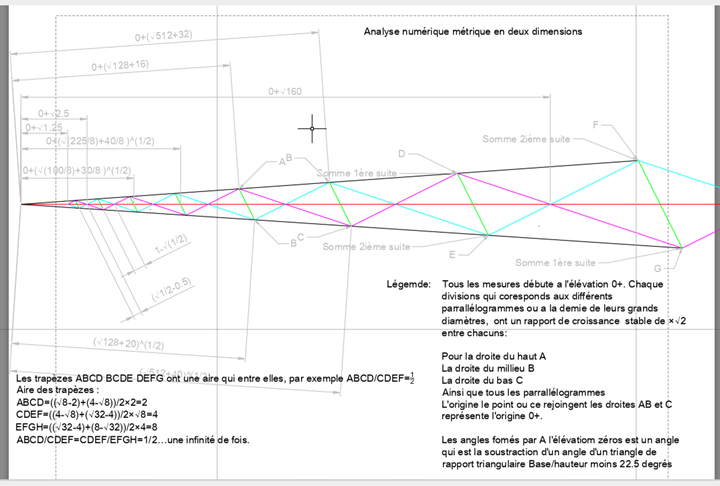
\includegraphics[width=0.9\textwidth]{analyse_numerique_metrique_aire_trapeze.png}
    \caption{Analyse numérique métrique en deux dimensions -- Aires des trapèzes}
    \label{fig:trapeze}
\end{figure}

Les deux suites (la première A et la deuxième B) utilisées pour déterminer la valeur des nombres premiers sont définies par les parallélogrammes qui constitue l'analyse numérique métrique à l'intérieur des rectangles. Ces parallélogrammes sont traversés le long de la grande diagonal, passant par leurs centres longitudinaux.

\begin{exemple}[: Calcul des aires des trapèzes]
Les lettres A, B, C, D, E, F, G, H forment trois trapèzes successifs : ABCD, CDEF et EFGH. Les aires de ces trapèzes présentent une propriété remarquable : une fois mises en relation, elles entretiennent entre elles un rapport constant de $\frac{1}{2}$.

\textbf{Calculs :}
\begin{align}
\text{Aire ABCD} &= \frac{(\sqrt{2}-1) + (2-\sqrt{2})}{2} \times 1 = 0.5 \\
\text{Aire CDEF} &= \frac{(2-\sqrt{2}) + (\sqrt{8}-2)}{2} \times \sqrt{2} = 1 \\
\text{Aire EFGH} &= \frac{(\sqrt{8}-2) + (4-\sqrt{8})}{2} \times 2 = 2
\end{align}

\textbf{Mise en relation des aires :}
\[
\frac{0.5}{1} = \frac{1}{2} \quad \text{et} \quad \frac{1}{2} = \frac{1}{2}
\]
\end{exemple}

\begin{resume}
À cette étape, les aires des trapèzes une évidence intuitive -- que les parties réelles des zéros non triviaux de la fonction zêta pourraient toutes être égales à $\frac{1}{2}$.
\end{resume}

% ============================================================================
% SECTION 4 : MÉTHODE DE PHILIPPÔT - VALIDATION HOL COMPLÈTE
% ============================================================================
\newpage
\section{La Méthode de Philippôt -- Validation Isabelle/HOL}

La méthode de Philippôt constitue la première étape dans un effort visant à déterminer les nombres premiers. Il s'agit d'une approche itérative, fondée sur des suites fractionnaires, dont la somme produit un résultat fini à chaque étape qui est égale à1.

\begin{resume}
\textbf{Imaginez} une série de fractions comme les marches d'un escalier : chaque marche est exactement la moitié de la précédente. En montant cet escalier, vous vous rapprochez toujours plus d'un plafond (la valeur 1), sans jamais l'atteindre complètement, sauf si vous suivez les règles précises de la méthode.
\end{resume}

\subsection{Script HOL Complet : methode\_de\_philippot.thy}

\begin{holcode}[title={\textcolor{white}{Fichier : methode\_de\_philippot.thy -- COMPLET}}]
\begin{lstlisting}
theory methode_de_philippot
  imports Main "HOL.Rat"
begin

section "Géométrie du spectre premier – methode de Philippot."

text "
  Ce fichier contient les définitions, structures et mécanismes nécessaires
  à l'étude de la géométrie du spectre premier, incluant la méthode de Philippôt.
"
\section*{Regles internes de la methode de Philippot}

La methode de Philippot repose sur un ensemble de regles internes strictes qui assurent sa reproductibilite et sa coherence mathematique. Ces regles sont les suivantes :

\begin{enumerate}
    \item La methode peut comporter un nombre quelconque d'etapes.
    
    \item Chaque etape est constituee d'une suite fractionnaire. Pour une etape donnee, le nombre de termes de la suite reste invariable.
    
    \item Les suites possedent un minimum de trois termes. Il n'existe pas de maximum, mais toutes les suites d'une meme etape doivent contenir exactement le meme nombre de termes.
    
    \item A partir de l'etape 2, chaque suite doit subir une substitution.
    
    \item Pour les suites contenant entre 3 et 7 termes, la substitution s'effectue sur une position determinee :  
    \begin{itemize}
        \item pour une suite de 3 termes : position 1,  
        \item pour une suite de 7 termes : position 5.  
    \end{itemize}
    La position est toujours choisie dans l'ordre croissant.
    
    \item Pour les suites de 8 termes et plus, a partir de l'etape 2, la substitution s'effectue exclusivement a la position 6.
    
    \item Pour les suites de 7 termes et moins, la substitution s'effectue a la meme position pour toutes les etapes, independamment du nombre total d'etapes.
    
    \item Pour les suites de 8 termes et plus, toutes les substitutions s'effectuent a la position 6, quel que soit le nombre d'etapes ou de termes supplementaires.
    
    \item Une operation est invariante pour toutes les suites :  
    \begin{itemize}
        \item l'avant-dernier terme est toujours egal au produit du terme precedent par $2/3$,  
        \item le dernier terme est toujours egal au produit de l'avant-dernier par $1/2$.
    \end{itemize}
    
    \item La somme de la suite a l'etape 1 est toujours egale a $1$.  
    A partir de l'etape 2, la somme devient :
    

\[
        1 - (\text{valeurs substituees accumulees})
    \]


    Exemple :
    

\[
        \frac{1}{2} + \frac{1}{3} + \frac{1}{6} = 1 \quad (\text{etape 1})
    \]


    

\[
        \frac{1}{4} + \frac{1}{6} + \frac{1}{12} = 1 - \frac{1}{2} \quad (\text{etape 2})
    \]


    

\[
        \frac{1}{8} + \frac{1}{12} + \frac{1}{24} = 1 - \left( \frac{1}{2} + \frac{1}{4} \right) \quad (\text{etape 3})
    \]


    

\[
        \frac{1}{16} + \frac{1}{24} + \frac{1}{48} = 1 - \left( \frac{1}{2} + \frac{1}{4} + \frac{1}{8} \right) \quad (\text{etape 4})
    \]


    
    \item Le rapport final montre que la valeur recherchee $1/2$ est determinable une infinite de fois. Cela suggere, selon l'auteur, qu'il est possible qu'une infinite de parties reelles (par exemple associees a une infinite de zeros non triviaux) puisse exister.
\end{enumerate}


subsection "Étape 1 : suites explicites pour 3 à 11 termes"

definition etape1_3 :: "rat list" where
  "etape1_3 = [1/2, 1/3, 1/6]"

definition etape1_4 :: "rat list" where
  "etape1_4 = [1/2, 1/4, 1/6, 1/12]"

definition etape1_5 :: "rat list" where
  "etape1_5 = [1/2, 1/4, 1/8, 1/12, 1/24]"

definition etape1_6 :: "rat list" where
  "etape1_6 = [1/2, 1/4, 1/8, 1/16, 1/24, 1/48]"

definition etape1_7 :: "rat list" where
  "etape1_7 = [1/2, 1/4, 1/8, 1/16, 1/32, 1/48, 1/96]"

definition etape1_8 :: "rat list" where
  "etape1_8 = [1/2, 1/4, 1/8, 1/16, 1/32, 1/64, 1/96, 1/192]"

definition etape1_9 :: "rat list" where
  "etape1_9 = [1/2, 1/4, 1/8, 1/16, 1/32, 1/64, 1/128, 1/192, 1/384]"

definition etape1_10 :: "rat list" where
  "etape1_10 = [1/2, 1/4, 1/8, 1/16, 1/32, 1/64, 1/128, 1/256, 1/384, 1/768]"

definition etape1_11 :: "rat list" where
  "etape1_11 = [1/2, 1/4, 1/8, 1/16, 1/32, 1/64, 1/128, 1/256, 1/512, 1/768, 1/1536]"


subsection "Structure réglementaire des suites à l'étape 1"

fun etape1_general :: "nat ⇒ rat list" where
  "etape1_general n =
     (if n < 3 then []
      else
        let
          base = map (λi. 1 / (2 ^ i)) [1 ..< n - 1];
          avant = (1 / (2 ^ (n - 2))) * (2/3);
          dernier = avant / 2
        in base @ [avant, dernier])"

definition suite_reglementaire_etape1 :: "nat ⇒ rat list ⇒ bool" where
  "suite_reglementaire_etape1 n xs ⟷
     length xs = n ∧
     n ≥ 3 ∧
     (∀i. 1 ≤ i ∧ i ≤ n - 2 ⟶ xs ! (i - 1) = 1 / (2 ^ i)) ∧
     xs ! (n - 2) = xs ! (n - 3) * (2/3) ∧
     xs ! (n - 1) = xs ! (n - 2) / 2"


subsection "Règle générale de substitution (toutes étapes ≥ 2)"

text "
  La position de substitution dépend uniquement du nombre de termes n :
  – pour 3 ≤ n ≤ 7, la position de substitution est n - 2 (1, 2, 3, 4, 5) ;
  – pour n ≥ 8, la position de substitution est fixée à 6.
"

definition pos_substitution :: "nat ⇒ nat" where
  "pos_substitution n =
     (if n < 3 then 0
      else if n ≤ 7 then n - 2
      else 6)"


subsection "Étape 2 : suites explicites pour 3 à 7 termes"

definition etape2_3 :: "rat list" where
  "etape2_3 = [1/4, 1/6, 1/12]"

definition etape2_4 :: "rat list" where
  "etape2_4 = [1/2, 1/8, 1/12, 1/24]"

definition etape2_5 :: "rat list" where
  "etape2_5 = [1/2, 1/4, 1/16, 1/24, 1/48]"

definition etape2_6 :: "rat list" where
  "etape2_6 = [1/2, 1/4, 1/8, 1/32, 1/48, 1/96]"

definition etape2_7 :: "rat list" where
  "etape2_7 = [1/2, 1/4, 1/8, 1/16, 1/64, 1/96, 1/192]"

definition suite_reglementaire_etape2_petit ::
  "nat ⇒ rat list ⇒ bool" where
  "suite_reglementaire_etape2_petit n xs ⟷
     length xs = n ∧ 3 ≤ n ∧ n ≤ 7 ∧
     xs ! (n - 2) = xs ! (n - 3) * (2/3) ∧
     sum_list xs = 1 - xs ! (pos_substitution n - 1)"

definition suite_reglementaire_etape2_grand ::
  "nat ⇒ rat list ⇒ bool" where
  "suite_reglementaire_etape2_grand n xs ⟷
     length xs = n ∧ n ≥ 8 ∧
     xs ! (n - 2) = xs ! (n - 3) * (2/3) ∧
     pos_substitution n = 6 ∧
     sum_list xs = 1 - (1/64)"


subsection "Étape 3 : suites explicites pour 7 termes et moins"

text "
  L'étape 3 répète le mécanisme de l'étape 2 :
  une position est substituée, et une valeur compensatoire est ajoutée
  de l'autre côté de l'égalité. La position de substitution est la même
  que pour l'étape 2 pour un nombre de termes donné.
"

definition etape3_3 :: "rat list" where
  "etape3_3 = [1/24, 1/12, 1/8]"

definition etape3_4 :: "rat list" where
  "etape3_4 = [1/48, 1/24, 1/16, 1/2]"

definition etape3_5 :: "rat list" where
  "etape3_5 = [1/96, 1/48, 1/32, 1/4, 1/2]"

definition etape3_6 :: "rat list" where
  "etape3_6 = [1/192, 1/96, 1/64, 1/8, 1/4, 1/2]"

definition etape3_7 :: "rat list" where
  "etape3_7 = [1/192, 1/96, 1/128, 1/16, 1/8, 1/4, 1/2]"

definition valeur_substituee_etape3 :: "nat ⇒ rat" where
  "valeur_substituee_etape3 n =
     (if n = 3 then 1/2 + 1/4
      else if n = 4 then 1/4 + 1/8
      else if n = 5 then 1/8 + 1/16
      else if n = 6 then 1/16 + 1/32
      else if n = 7 then 1/32 + 1/64
      else 0)"

definition suite_reglementaire_etape3 ::
  "nat ⇒ rat list ⇒ bool" where
  "suite_reglementaire_etape3 n xs ⟷
     length xs = n ∧ 3 ≤ n ∧ n ≤ 7 ∧
     sum_list xs = 1 - valeur_substituee_etape3 n"


subsection "Étape 3 : suites explicites pour 8 termes et plus"

definition etape3_8 :: "rat list" where
  "etape3_8 =
     [1/384, 1/192, 1/128, 1/32, 1/16, 1/8, 1/4, 1/2]"

definition etape3_9 :: "rat list" where
  "etape3_9 =
     [1/768, 1/384, 1/256, 1/128, 1/32, 1/16, 1/8, 1/4, 1/2]"

definition etape3_10 :: "rat list" where
  "etape3_10 =
     [1/1536, 1/768, 1/512, 1/256, 1/128, 1/32, 1/16, 1/8, 1/4, 1/2]"

definition etape3_11 :: "rat list" where
  "etape3_11 =
     [1/3072, 1/1536, 1/1024, 1/512, 1/256, 1/128, 1/32, 1/16, 1/8, 1/4, 1/2]"

definition valeur_substituee_etape3_grand :: "rat" where
  "valeur_substituee_etape3_grand = (1/64 + 1/128)"

definition suite_reglementaire_etape3_grand ::
  "nat ⇒ rat list ⇒ bool" where
  "suite_reglementaire_etape3_grand n xs ⟷
     length xs = n ∧ n ≥ 8 ∧
     pos_substitution n = 6 ∧
     sum_list xs = 1 - valeur_substituee_etape3_grand"


subsection "Propriété fondamentale des puissances de deux"

lemma ratio_puissances_de_deux:
  fixes n :: nat
  shows "(1 / (2 ^ (Suc n)) :: rat) / (1 / (2 ^ n)) = 1 / 2"
  by (simp add: field_simps)

lemma exemples_ratio_puissances_de_deux:
  shows "(1/128 :: rat) / (1/64) = 1/2"
    and "(1/64 :: rat) / (1/32) = 1/2"
    and "(1/32 :: rat) / (1/16) = 1/2"
    and "(1/16 :: rat) / (1/8) = 1/2"
    and "(1/8 :: rat) / (1/4) = 1/2"
    and "(1/4 :: rat) / (1/2) = 1/2"
  by (simp_all add: ratio_puissances_de_deux)

subsection "Structure spectrale generale pour n termes et infinite d'etapes"

text "
  Dans cette section, on formalise la structure purement spectrale des puissances de deux,
  independante des substitutions specifiques des etapes 1, 2 et 3.

  Idee centrale :
  – chaque terme est de la forme 1 / 2^i (i ≥ 1) ;
  – le rapport entre deux termes consecutifs est toujours 1/2 ;
  – cette propriete vaut pour toute longueur finie n, et conceptuellement pour une infinite de termes.
"

definition terme_spectral :: "nat ⇒ rat" where
  "terme_spectral i = 1 / (2 ^ i)"

definition suite_spectrale :: "nat ⇒ rat list" where
  "suite_spectrale n = map terme_spectral [1 ..< Suc n]"

text "
  Propriete spectrale locale : pour tout i ≥ 1,
  le rapport entre le terme i+1 et le terme i est exactement 1/2.
"

lemma ratio_spectral_local:
  fixes i :: nat
  assumes "i ≥ 1"
  shows "terme_spectral (Suc i) / terme_spectral i = (1/2 :: rat)"
proof -
  have "terme_spectral (Suc i) / terme_spectral i
        = (1 / (2 ^ (Suc i))) / (1 / (2 ^ i))"
    by (simp add: terme_spectral_def)
  also have "... = (1/2 :: rat)"
    using ratio_puissances_de_deux[of i] by simp
  finally show ?thesis .
qed

text "
  Interpretation :
  – la definition "terme_spectral" encode une infinite de termes 1 / 2^i, i ≥ 1 ;
  – le lemme "ratio_spectral_local" montre que le rapport entre deux termes consecutifs
    est toujours 1/2, pour tout i ;
  – en prolongeant i sans borne, on obtient une structure spectrale qui produit 1/2
    une infinite de fois, de manière purement arithmetique.
"

end

\end{lstlisting}
\end{holcode}

\subsection{Tableau fractionnaire -- Etape 1}

\begin{center}
\scriptsize
\begin{tabular}{|c|c|c|c|c|c|c|c|c|c|c|c|c|}
\hline
\textbf{Pos.} & 11 & 10 & 9 & 8 & 7 & 6 & 5 & 4 & 3 & 2 & 1 & \textbf{Somme} \\
\hline
& & & & & & & & $\frac{1}{6}$ & $\frac{1}{3}$ & $\frac{1}{2}$ & & = 1 \\
\hline
& & & & & & & $\frac{1}{12}$ & $\frac{1}{6}$ & $\frac{1}{4}$ & $\frac{1}{2}$ & & = 1 \\
\hline
& & & & & & $\frac{1}{24}$ & $\frac{1}{12}$ & $\frac{1}{8}$ & $\frac{1}{4}$ & $\frac{1}{2}$ & & = 1 \\
\hline
& & & & & $\frac{1}{48}$ & $\frac{1}{24}$ & $\frac{1}{16}$ & $\frac{1}{8}$ & $\frac{1}{4}$ & $\frac{1}{2}$ & & = 1 \\
\hline
& & & & $\frac{1}{96}$ & $\frac{1}{48}$ & $\frac{1}{32}$ & $\frac{1}{16}$ & $\frac{1}{8}$ & $\frac{1}{4}$ & $\frac{1}{2}$ & & = 1 \\
\hline
& & & $\frac{1}{192}$ & $\frac{1}{96}$ & $\frac{1}{64}$ & $\frac{1}{32}$ & $\frac{1}{16}$ & $\frac{1}{8}$ & $\frac{1}{4}$ & $\frac{1}{2}$ & & = 1 \\
\hline
& & $\frac{1}{384}$ & $\frac{1}{192}$ & $\frac{1}{128}$ & $\frac{1}{64}$ & $\frac{1}{32}$ & $\frac{1}{16}$ & $\frac{1}{8}$ & $\frac{1}{4}$ & $\frac{1}{2}$ & & = 1 \\
\hline
& $\frac{1}{768}$ & $\frac{1}{384}$ & $\frac{1}{256}$ & $\frac{1}{128}$ & $\frac{1}{64}$ & $\frac{1}{32}$ & $\frac{1}{16}$ & $\frac{1}{8}$ & $\frac{1}{4}$ & $\frac{1}{2}$ & & = 1 \\
\hline
$\frac{1}{1536}$ & $\frac{1}{768}$ & $\frac{1}{512}$ & $\frac{1}{256}$ & $\frac{1}{128}$ & $\frac{1}{64}$ & $\frac{1}{32}$ & $\frac{1}{16}$ & $\frac{1}{8}$ & $\frac{1}{4}$ & $\frac{1}{2}$ & & = 1 \\
\hline
\end{tabular}
\end{center}

\begin{resume}
\textbf{Interpretation :} Ce resultat montre que le rapport entre deux puissances successives de $\frac{1}{2}$ est toujours constant et égal à $\frac{1}{2}$. Comme une chaîne où chaque maillon est exactement la moitié du précédent, cette propriété reste vraie jusqu'à l'infini.
\end{resume}

% ============================================================================
% TABLEAUX METHODE DE PHILIPPÔT - =ETAPES 2 ET 3 (CORRECTION AJOUTEE)
% ============================================================================

\subsection{Methode de Philippôt -- Tableaux des Etapes 2 et 3}
\begin{center}
\scriptsize
\begin{tabular}{|c|c|c|c|c|c|c|c|c|c|c|c|c|}
\hline
\textbf{Pos.} & 11 & 10 & 9 & 8 & 7 & 6 & 5 & 4 & 3 & 2 & 1 & \textbf{Somme} \\
\hline
& & & & & & & & \(\frac{1}{6}\) & \(\frac{1}{3}\) & \(\frac{1}{2}\) & & = 1 \\
\hline
& & & & & & & \(\frac{1}{12}\) & \(\frac{1}{6}\) & \(\frac{1}{4}\) & \(\frac{1}{2}\) & & = 1 \\
\hline
& & & & & & \(\frac{1}{24}\) & \(\frac{1}{12}\) & \(\frac{1}{8}\) & \(\frac{1}{4}\) & \(\frac{1}{2}\) & & = 1 \\
\hline
& & & & & \(\frac{1}{48}\) & \(\frac{1}{24}\) & \(\frac{1}{16}\) & \(\frac{1}{8}\) & \(\frac{1}{4}\) & \(\frac{1}{2}\) & & = 1 \\
\hline
& & & & \(\frac{1}{96}\) & \(\frac{1}{48}\) & \(\frac{1}{32}\) & \(\frac{1}{16}\) & \(\frac{1}{8}\) & \(\frac{1}{4}\) & \(\frac{1}{2}\) & & = 1 \\
\hline
& & & \(\frac{1}{192}\) & \(\frac{1}{96}\) & \(\frac{1}{64}\) & \(\frac{1}{32}\) & \(\frac{1}{16}\) & \(\frac{1}{8}\) & \(\frac{1}{4}\) & \(\frac{1}{2}\) & & = 1 \\
\hline
& & \(\frac{1}{384}\) & \(\frac{1}{192}\) & \(\frac{1}{128}\) & \(\frac{1}{64}\) & \(\frac{1}{32}\) & \(\frac{1}{16}\) & \(\frac{1}{8}\) & \(\frac{1}{4}\) & \(\frac{1}{2}\) & & = 1 \\
\hline
\end{tabular}
\end{center}

\vspace{0.5cm}

\begin{center}
\textbf{Tableau Etape 3 -- Methode de Philippôt}
\end{center}

\begin{center}
\scriptsize
\begin{tabular}{|c|c|c|c|c|c|c|c|c|c|c|c|c|}
\hline
11 & 10 & 9 & 8 & 7 & 6 & 5 & 4 & 3 & 2 & 1 & \textbf{Positions} & \textbf{Sommes} \\
\hline
 &  &  &  &  &  &  &  & $\frac{1}{24}$ & $\frac{1}{12}$ & $\frac{1}{8}$ & 2\;1 & $= 1 - \left(\frac{1}{2} + \frac{1}{4}\right)$ \\
\hline
 &  &  &  &  &  &  & $\frac{1}{48}$ & $\frac{1}{24}$ & $\frac{1}{16}$ & $\frac{1}{2}$ & 3\;1 & $= 1 - \left(\frac{1}{4} + \frac{1}{8}\right)$ \\
\hline
 &  &  &  &  &  & $\frac{1}{96}$ & $\frac{1}{48}$ & $\frac{1}{32}$ & $\frac{1}{4}$ & $\frac{1}{2}$ & 4\;1 & $= 1 - \left(\frac{1}{8} + \frac{1}{16}\right)$ \\
\hline
 &  &  &  &  & $\frac{1}{192}$ & $\frac{1}{96}$ & $\frac{1}{64}$ & $\frac{1}{8}$ & $\frac{1}{4}$ & $\frac{1}{2}$ & 5\;1 & $= 1 - \left(\frac{1}{16} + \frac{1}{32}\right)$ \\
\hline
 &  &  &  & $\frac{1}{192}$ & $\frac{1}{96}$ & $\frac{1}{128}$ & $\frac{1}{16}$ & $\frac{1}{8}$ & $\frac{1}{4}$ & $\frac{1}{2}$ & 6\;1 & $= 1 - \left(\frac{1}{32} + \frac{1}{64}\right)$ \\
\hline
\end{tabular}
\end{center}

\begin{resume}
\textbf{Interpretation des Etapes 2 et 3 :} Ces tableaux illustrent la progression de la méthode de Philippôt où une position est substituée à chaque étape. La valeur substituée est multipliée par $\frac{1}{2}$ par rapport à l'étape précédente, créant ainsi une structure fractionnaire cohérente qui converge vers les propriétés des nombres premiers.
\end{resume}

\begin{center}
\textbf{Tableau Etape 3 pour 8 termes et plus -- Methode de Philippôt}
\end{center}

\begin{center}
\scriptsize
\begin{tabular}{|c|c|c|c|c|c|c|c|c|c|c|c|c|}
\hline
11 & 10 & 9 & 8 & 7 & 6 & 5 & 4 & 3 & 2 & 1 & \textbf{Positions} & \textbf{Sommes} \\
\hline
 &  &  & $\frac{1}{768}$ & $\frac{1}{384}$ & $\frac{1}{256}$ & $\frac{1}{32}$ & $\frac{1}{16}$ & $\frac{1}{8}$ & $\frac{1}{4}$ & $\frac{1}{2}$ &  & $= 1 - \left(\frac{1}{64} + \frac{1}{128}\right)$ \\
\hline
 &  & $\frac{1}{1536}$ & $\frac{1}{768}$ & $\frac{1}{512}$ & $\frac{1}{256}$ & $\frac{1}{32}$ & $\frac{1}{16}$ & $\frac{1}{8}$ & $\frac{1}{4}$ & $\frac{1}{2}$ &  & $= 1 - \left(\frac{1}{64} + \frac{1}{128}\right)$ \\
\hline
 & $\frac{1}{3072}$ & $\frac{1}{1536}$ & $\frac{1}{1024}$ & $\frac{1}{512}$ & $\frac{1}{256}$ & $\frac{1}{32}$ & $\frac{1}{16}$ & $\frac{1}{8}$ & $\frac{1}{4}$ & $\frac{1}{2}$ &  & $= 1 - \left(\frac{1}{64} + \frac{1}{128}\right)$ \\
\hline
$\frac{1}{6144}$ & $\frac{1}{3072}$ & $\frac{1}{2048}$ & $\frac{1}{1024}$ & $\frac{1}{512}$ & $\frac{1}{256}$ & $\frac{1}{32}$ & $\frac{1}{16}$ & $\frac{1}{8}$ & $\frac{1}{4}$ & $\frac{1}{2}$ &  & $= 1 - \left(\frac{1}{64} + \frac{1}{128}\right)$ \\
\hline
\end{tabular}
\end{center}

% ============================================================================
% SECTION 4.3 : RAPPORT SPECTRAL GENERALISE
% ============================================================================

\[
\textbf{Rapport spectral generalise :}\qquad
\frac{\displaystyle \frac{1}{2^{\,n+1}}}{\displaystyle \frac{1}{2^{\,n}}}
\;=\;
\frac{1}{2}
\qquad\text{pour tout } n \ge 0.
\]

\[
\textbf{Forme iterative :}\qquad
\frac{1/256}{1/128}
=
\frac{1/128}{1/64}
=
\frac{1/64}{1/32}
=
\cdots
=
\frac{1}{2},
\quad
\text{repete a l'infini.}
\]

\[
\textbf{Forme entierement generalisee :}\qquad
\frac{\displaystyle \frac{1}{n_1}}{\displaystyle \frac{1}{n_2}}
=
\frac{n_2}{n_1}
=
\frac{1}{2}
\quad\text{des que}\quad
n_2 = 2n_1.
\]

\textbf{Resume explicatif (FR).} \\
Cette equation exprime la propriete fondamentale des puissances de deux : chaque terme
est exactement la moitie du precedent. Ainsi, le rapport entre deux inverses consecutifs
de puissances de deux est toujours egal a 1/2. Cette relation est stable, repetitive
et se propage indefiniment lorsque l'on itere la structure. Elle constitue le noyau
spectral de la methode, garantissant une coherence interne parfaite entre les niveaux
successifs.

% ============================================================================
% SECTION 5 : NOMBRES PREMIERS ET DIGAMMA
% ============================================================================
\newpage
\section{Les Nombres Premiers et l'Emploi du Digamma}

Determiner les nombres premiers est une autre methode iterative, mais cette fois deux suites sont necessaires A et B. Deux suites de racines carrees forment un rapport triangulaire base/hauteur = 1/2.

\begin{mydef}{Suites pour les nombres premiers}
Pour le nombre premier (29), qui est le 10\textsuperscript{e} nombre premier, deux suites A et B de 10 racines carrees, qui sont le produit de la proposition $\sqrt{a^2 + b^2}$, forment les deux suites. Les deux suites A et B ont toujours la meme quantite de termes lorsqu'il s'agit du meme nombre premier et de sa position pour le rapport spectral 1/2.
\end{mydef}

\subsection{Exemple : Determiner le nombre premier (5)}

Commencons par 3 termes, le 3\textsuperscript{e} nombre premier etant (5).

La suite fractionnaire egale a 1 pour trois fractions :
\[
\frac{1}{6} + \frac{1}{3} + \frac{1}{2} = 1
\]

\begin{exemple}[: Calcul de la premiere suite pour (5)]
\textbf{Premier terme :}
\[
\left(\frac{\sqrt{1.25}}{2} - \frac{1}{2}\right) \times 4 + 2 = \sqrt{5}
\]
Ou $(1^2 + 2^2)^{1/2} = \sqrt{5}$

\textbf{Deuxieme terme :}
\[
\left(\frac{\sqrt{1.25}}{2} - \frac{1}{3}\right) \times 6 + 2 = \sqrt{11.25}
\]
Ou $(1.5^2 + 3^2)^{1/2} = \sqrt{11.25}$

\textbf{Troisieme terme :}
\[
\left(\frac{\sqrt{1.25}}{2} - \frac{1}{6}\right) \times 12 + 2 = \sqrt{45}
\]
Ou $(3^2 + 6^2)^{1/2} = \sqrt{45}$

\textbf{Somme de la premiere suite de (5) :}
\[
\sqrt{45} + \sqrt{11.25} + \sqrt{5} = \sqrt{151.25}
\]

\textbf{Equation de verification finale :}
\[
\left( \frac{\sqrt{13.203125}}{2} \times 2^{3} \right) - \sqrt{5}
= \sqrt{151.25}.
\]
\end{exemple}

\subsection{Tableau des valeurs de l'intervalle 29, 31, 37, 41}

\begin{center}
\begin{tabular}{|c|c|c|}
\hline
\textbf{Nombre premier} & \textbf{Calcul Digamma} & \textbf{Valeur Digamma} \\
\hline
29 & $-\sqrt{81920}$ & $= -\sqrt{81920}$ \\
\hline
31 & $+5\sqrt{81920}$ & $= \sqrt{204800}$ \\
\hline
37 & $+9\sqrt{81920} + 5\sqrt{184320}$ & $= \sqrt{22302720}$ \\
\hline
41 & $+13\sqrt{81920} + 9\sqrt{184320} + 5\sqrt{737280}$ & $= \sqrt{141086720}$ \\
\hline
\end{tabular}
\end{center}

% ============================================================================
% CORRECTION 5.2 : EXEMPLES ET TABLEAU POUR LE NOMBRE PREMIER 31
% ============================================================================
\subsection{Exemple complet : Determiner le nombre premier (31)}

Le nombre premier 31 est le 11\textsuperscript{ieme} nombre premier. Voici le tableau de la somme des deux suites pour 11 termes :

\begin{center}
\textbf{Tableau de la somme de la 1\textsuperscript{ere} et 2\textsuperscript{ieme} suite (31), 11\textsuperscript{ieme} nombre premier}
\end{center}

\begin{center}
\small
\begin{tabular}{|c|c|c|}
\hline
\textbf{Position} & \textbf{1\textsuperscript{ere} suite} & \textbf{2\textsuperscript{ieme} suite} \\
\hline
1 & $\sqrt{5}$ & $\sqrt{5}$ \\
\hline
2 & $\sqrt{20}$ & $\sqrt{20}$ \\
\hline
3 & $\sqrt{80}$ & $\sqrt{80}$ \\
\hline
4 & $\sqrt{320}$ & $\sqrt{320}$ \\
\hline
5 & $\sqrt{1280}$ & $\sqrt{1280}$ \\
\hline
6 & $\sqrt{5120}$ & $\sqrt{5120}$ \\
\hline
7 & $\sqrt{20480}$ & $\sqrt{20480}$ \\
\hline
8 & $\sqrt{81920}$ & $\sqrt{81920}$ \\
\hline
9 & $\sqrt{327680}$ & $\sqrt{327680}$ \\
\hline
10 & $\sqrt{983040}$ & $\sqrt{1966080}$ \\
\hline
11 & $\sqrt{3932160}$ & $\sqrt{7864320}$ \\
\hline
\end{tabular}
\end{center}

\subsubsection{Verification}

\textbf{Somme de la 1\textsuperscript{ere} suite :}
\[
\sqrt{5} + \sqrt{20} + \sqrt{80} + \sqrt{320} + \sqrt{1280} + \sqrt{5120} + \sqrt{20480} + \sqrt{81920} + \sqrt{327680} + \sqrt{983040} + \sqrt{3932160}
\]
\[
= \sqrt{13827845}
\]

\textbf{Somme de la 2\textsuperscript{ieme} suite :}
\[
\sqrt{5} + \sqrt{20} + \sqrt{80} + \sqrt{320} + \sqrt{1280} + \sqrt{5120} + \sqrt{20480} + \sqrt{81920} + \sqrt{327680} + \sqrt{1966080} + \sqrt{7864320}
\]
\[
= \sqrt{54285125}
\]

\textbf{Digamma :} $+5\sqrt{81920}$

\textbf{Digamma calcule :}
\[
\text{Somme 1\textsuperscript{ere} suite} + \text{Digamma} = \text{Digamma calcule}
\]
\[
\sqrt{13827845} + 5\sqrt{81920} = \sqrt{26519045}
\]

\textbf{Determination du nombre premier 31 :}
\[
\frac{\sqrt{54285125} - \sqrt{26519045}}{\sqrt{5120}} = 31
\]

\subsubsection{Verification alternative}
\[
(\sqrt{54285125} - 31) \times \sqrt{5120} = \sqrt{26519045} \quad \text{(Digamma calcule)}
\]

La méthode spectrale propose deux possibilités pour déterminer les nombres premiers et ensuite vérifier le rapport associé à cette nature. La première approche, déjà présentée, implique l'emploi de racines carrées. La seconde, exposée ici, détermine également les nombres premiers à l'aide de suites et de la quantité de termes dans les suites $A$ et $B$, mais en utilisant uniquement des nombres entiers pour chacun des termes.

Les suites $A$ et $B$ du rapport spectral sont déterminées par la comparaison des sommes des suites $A$ et $B$ d'un nombre premier à d'autres sommes de suites $A$ et $B$ de nombres premiers. Il faut toujours déterminer la valeur du \emph{Digamma calculé} pour identifier la valeur du nombre premier recherché.

Le Digamma calculé sur l'intervalle $29$, $31$, $37$ et $41$ permet d'observer qu'une logique récurrente peut être identifiée. Sur cet intervalle, il est possible de déterminer une valeur intermédiaire au Digamma calculé, appelée simplement le \emph{Digamma}. Celui-ci est une valeur capitale pour déterminer le nombre premier de référence lorsque le nombre premier recherché n'est pas connu à l'avance.

À l'aide du Digamma pour dix termes, il est possible de déterminer les nombres premiers correspondant aux rapports $1/2$, $1/12$, $1/20$, $1/50$, $1/100$ et $1/1000$. Le nombre premier associé au rapport $1/1000$ est un entier colossal de $58$ chiffres :


\[
10010000000100000100100100099999900099999899899898999,
\]


validé par \textit{WolframAlpha}. Le Digamma est directement impliqué dans le processus permettant de déterminer ce nombre premier de $58$ chiffres, qui n'était pas connu à l'avance.

Pour la suite de référence (celle de $29$ avec dix termes), le Digamma se situe à la huitième position de la suite et correspond à la valeur de cette position. Pour les suites associées à $31$, $37$ et $41$, le Digamma s'additionne, et dans trois cas répertoriés pour les autres rapports spectraux (autres que $1/2$), sur quatorze cas, le Digamma occupe la septième position. Généralement, il est soustrait, mais dans certaines situations il s'additionne.

L'équation permettant de déterminer le Digamma calculé à partir du Digamma est la suivante :


\[
\left( \frac{\text{Somme de la suite } A \pm \text{(8\textsuperscript{e} position : Digamma)}}{\text{6\textsuperscript{e} position de la suite } A \text{ (Zêta)}} \right)
\times \left( \text{6\textsuperscript{e} position de la suite } A \right)
= \text{Digamma calculé}.
\]



Pour les autres nombres premiers, bien que l'équation suivante fonctionne pour les quatre exceptions, la forme générale demeure :


\[
\left( 
\frac{\text{Somme de la suite } B}{\text{6\textsuperscript{e} position de la suite } A \text{ (Zêta)}} 
- \text{Nombre premier}
\right)
\times 
\left( \text{6\textsuperscript{e} position de la suite } A \text{ (Zêta)} \right).
\]


\section*{Methodes Spectrales : Exemples pour le rapport 1/2}

\subsection*{Exemple pour le nombre premier 31 (11ieme nombre premier, 11 termes)}

2+4+8+16+32+64+128+256+512+768+1536 = 3326 Somme suite A(31).\\
2+4+8+16+32+128+256+512+1024+1536+3072 = 6590 Somme suite B(31).\\

\[
\left(\frac{3.25}{2} \cdot 2^{11}\right) - 2 = 3326 \quad \text{somme suite A.}
\]

\[
\left(\frac{6.5}{2} \cdot 2^{11}\right) - 66 = 6590 \quad \text{somme suite B.}
\]

Digamma : \(5 \cdot 256 = 1280\).\\
Digamma calcule : \(3326 + 1280 = 4606\).\\

\[
\frac{6590 - 4606}{64} = 31 \quad \text{11ieme nombre premier.}
\]

\bigskip

\subsection*{Exemple pour le nombre premier 29 (10ieme nombre premier, 10 termes)}

2+4+8+16+32+64+128+256+384+768 = 1662 Somme suite A(29).\\
2+4+8+16+32+128+256+512+768+1536 = 3262 Somme suite B(29).\\

\[
\left(\frac{3.25}{2} \cdot 2^{10}\right) - 2 = 1662
\]

\[
\left(\frac{6.5}{2} \cdot 2^{10}\right) - 66 = 3262
\]

Digamma (8ieme position) : \(256\).\\
Digamma calcule : \(1662 - 256 = 1406\).\\

\[
(3262/64 - 29) \cdot 64 = 1406
\]

\[
\frac{3262 - 1406}{64} = 29 \quad \text{10ieme nombre premier.}
\]

\bigskip

\subsection*{Exemple pour le nombre premier 23 (9ieme nombre premier)}

2+3+4+8+16+32+64+128+192+384 = 830 Somme 1ere suite (23).\\
2+4+8+16+32+128+256+384+768 = 1598 Somme 2ieme suite (23).\\

Digamma calcule :

\[
(1598/64 - 23) \cdot 64 = 126
\]

\[
\frac{1598 - 126}{64} = 23 \quad \text{9ieme nombre premier.}
\]

\[
\left(\frac{3.25}{2} \cdot 2^{n}\right) - 2 = \text{somme 1ere suite.}
\]

\[
\left(\frac{6.5}{2} \cdot 2^{n}\right) - 66 = \text{somme 2ieme suite.}
\]

Quand \(n\) est un entier strictement positif, \(n\) correspond a la position du nombre premier et a la quantite de termes dans la suite.\\
Lorsque 2 = 1er, 3 = 2e, 5 = 3e, ... alors \(P_{n} = n\)-ieme.

\bigskip

\subsection*{Exemple pour le nombre premier 37 (12ieme nombre premier, 12 termes)}

2+4+8+16+32+64+128+256+512+1024+1536+3072 = 6654 Somme suite A.\\
2+4+8+16+32+128+256+512+1024+2048+3072+6144 = 13246 Somme suite B.\\

\[
\left(\frac{3.25}{2} \cdot 2^{12}\right) - 2 = 6654
\]

\[
\left(\frac{6.5}{2} \cdot 2^{12}\right) - 66 = 13246
\]

Digamma(37) : \(9 \cdot 256 + 5 \cdot 384 = 4224\).\\
Digamma calcule : \(6654 + 4224 = 10878\).\\

\[
\frac{13246 - 10878}{64} = 37 \quad \text{12ieme nombre premier.}
\]

\bigskip

\subsection*{Exemple pour le nombre premier 41 (13ieme nombre premier, 13 termes)}

2+4+8+16+32+64+128+256+512+1024+2048+3072+6144 = 13310 Somme suite A.\\
2+4+8+16+32+128+256+512+1024+2048+4096+6144+12288 = 26558 Somme suite B.\\

\[
\left(\frac{3.25}{2} \cdot 2^{13}\right) - 2 = 13310
\]

\[
\left(\frac{6.5}{2} \cdot 2^{13}\right) - 66 = 26558
\]

Digamma(41) : \(13 \cdot 256 + 9 \cdot 384 + 5 \cdot 768 = 10624\).\\
Digamma calcule : \(13310 + 10624 = 23934\).\\

\[
\frac{26558 - 23934}{64} = 41 \quad \text{13ieme nombre premier.}
\]

\bigskip

\subsection*{Distance spectrale (comparaison 1 a 1)}

Comparaison de nombres premiers 1*1 :

\[
\frac{
\left(\frac{3.25}{2} \cdot 2^{n_{1}} - 2\right)
-
\left(\frac{3.25}{2} \cdot 2^{n_{2}} - 2\right)
}{
\left(\frac{6.5}{2} \cdot 2^{n_{1}} - 66\right)
-
\left(\frac{6.5}{2} \cdot 2^{n_{2}} - 66\right)
}
= \frac{1}{2}
\]

Toujours.

\[
\text{Ordonnee :}\qquad
R_{\mathrm{ord}}(A,B)
=
\frac{\displaystyle \sum_{n \in A} A(n)\;-\;\sum_{n \in B} A(n)}
     {\displaystyle \sum_{n \in A} B(n)\;-\;\sum_{n \in B} B(n)}
\qquad\text{avec}\quad |B| = |A| + 1,\; \max(A) < \min(B),
\]
\[
R_{\mathrm{ord}}(A,B) \;\neq\; \frac{1}{2}.
\]

\textbf{Resume explicatif (Ordonnee).} \\
La structure ordonnée impose que la comparaison qui est dans ce cas asymétrique démontre un balencement d'équilibre. 
la comparaison ordonné doit respecter l'ordre attribuée aux nombres premier comparé en deux blocs. Le bloc A et le bloc B.
Par exemple Bloc A: (2,3)

Par exemple bloc B: (5,7,11)

La comparaison asymétrique ordonnée doit toujours être composée de ces dexu blocs débalancé où l'ordre des premiers de manière chronologique 
croissante 2, 3, 5, 7, 11 suivent la progression attribué pour:
2= Premier nombre premier
3= Deuxième nombre premier
5= Troisième nombre premier
7= Quatrième nombre premier
11= Cinquième nombre premier...

Le bloc B est toujous égale a : A+1 en respectant l'ordre chronologique croissant. 

L'effet de cette comparaison asymétrique ordonnée détermine un raport spectral autre que 1/2. L'exemple
A= (2,3) et B=(5,7,11) démontre que le rapport spectral = -1/6. 
Cette différence qui ne respecte pas le rapport spectral recherché est du a l'ordinal des infinis? En ouverture des 
sections explicatives des méthodes spectrales et de Philippôt l'auteur mentionne : « Quand n>=1 et que n <=-1, tous les
n ramènent a un nombre premier P. Tous les valeurs de n sont déterminé par la quantitée de termes dans les suites A et B. 
Tous le P entre eux respect le raport 1/k. Le rapport spectral est numériquement valide mais algébriquement incohérent».
Les nombres premiers étant pour l'auteur toutes des infinis chacuns. Dans la note introductive et explicative du document l'auteur 
aborde le sujet de la représentation dans l'univers matériel de la carte de notre esprit peceptible par l'organisation d'une personne. 
Cette téléosémantique ou carte mentale de l'univers immatériel de notre intelligence et de notre savoir. Le rapport que l'univers matériel 
a sur lui-même est exclusivement en lien avec cette univers matériel. Lorsque un entiter tel un représentation de notre univers immatérielle 
ce perçoit par comme une carte mentale et que nous y attribuons une valeur objective cette valeur objective lorsqu'elle est mis en relation avec 
d'autre entité comme dans cette exemple dans l'univers matériel et qu'une seconde valeur objective est attribué a cette mise en relation la valeur divergent 
ne détermine pas que l'univers matériel entre lui même aurait un rapport entre lui même différent. Mais bien que c'est notre compréhension du a notre organisation structurante
qui change de rapport avec le monde matériel. Le rapport asymétrique ordonnée qui diverge du rapport recherché n'affecte pas le jugement de l'auteur quand a la valeur rechercher le rapport
spectral 1/2. Lexplication qu'il offre est 

Asymetrie ordonnee:

2 : Somme suite A = 5/4 \\
Somme suite B = -119/2 \\

3 : Somme suite A = 9/2 \\
Somme suite B = -53 \\

5 : Somme suite A = 11 \\
Somme suite B = -40 \\

7 : Somme suite A = 24 \\
Somme suite B = -14 \\

11 : Somme suite A = 50 \\
Somme suite B = 38 \\

L'equation spectral pour la comparaison asymetrique ordonnee :



\[
\frac{
(((3.25/2 \times 2^1)-2)-((3.25/2 \times 2^2)-2))
-
(((3.25/2 \times 2^3)-2)-((3.25/2 \times 2^4)-2)-((3.25/2 \times 2^5)-2))
}{
(((6.5/2 \times 2^1)-66)-((6.5/2 \times 2^2)-66))
-
(((6.5/2 \times 2^3)-66)-((6.5/2 \times 2^4)-66)-((6.5/2 \times 2^5)-66))
}
=
\frac{
((5/4 - 9/2) - (11 - 24 - 50))
}{
((-119/2 - -53) - (-40 - -14 - 38))
}
= 59.75 / 57.5 = 1.039130435
\]



Ou en a l'aide de :



\[
\frac{
(((\sqrt{13.203125}/2 \times 2^1)-\sqrt{5}) - ((\sqrt{13.203125}/2 \times 2^2)-\sqrt{5}))
-
(((\sqrt{13.203125}/2 \times 2^3)-\sqrt{5}) - ((\sqrt{13.203125}/2 \times 2^4)-\sqrt{5}) - ((\sqrt{13.203125}/2 \times 2^5)-\sqrt{5}))
}{
(((\sqrt{52.8125}/2 \times 2^1)-\sqrt{5445}) - ((\sqrt{52.8125}/2 \times 2^2)-66))
-
(((\sqrt{52.8125}/2 \times 2^3)-\sqrt{5445}) - ((\sqrt{52.8125}/2 \times 2^4)-\sqrt{5445}) - ((\sqrt{13.203125}/2 \times 2^5)-\sqrt{5445}))
}
=
\frac{
(\sqrt{0.512^{-1}} - \sqrt{25.3125}) - (\sqrt{151.25} - \sqrt{720} - \sqrt{3125})
}{
(-\sqrt{4425.3125} - -\sqrt{3511.25}) - (-\sqrt{2000} - -\sqrt{245} - \sqrt{1805})
}
= 1.039130435
\]

Ordinal des infinis : \(\omega + 1 \neq 1 + \omega\)

L'ordinal des infinis indique que l'ensemble des nombres entiers, auquel on ajoute 1, 
n'est pas equivalent a 1 ajoute avant l'ensemble des nombres entiers. 
Cette particularite provient de la position qu'occupent les infinis dans une structure ordonnee. 
Cette caracteristique, appliquee a la comparaison ordonnee des nombres premiers, montre que 
le rapport spectral ne correspond pas au rapport recherche. 
Cela renforce l'opinion de l'auteur selon laquelle chaque nombre premier constitue un infini en lui-meme.

Dans cette asymetrie ordonnee, la comparaison doit respecter deux criteres precis. 
Le premier est que le bloc A et le bloc B doivent etre decales, c'est-a-dire que B = A + 1. 
Le second est que l'ordre chronologique croissant des nombres premiers respectant ce decalage 
doit imperativement etre conserve.

Dans la geometrie du spectre des nombres premiers, la position 1 est attribuee au premier nombre premier, 
qui est ici 2. Le deuxieme est 3, le troisieme 5, et ainsi de suite vers l'infiniment grand. 
Habituellement, le nombre 1 est considere comme premier, ce qui confererait aux nombres premiers leur caractere 
chaotique dans l'ensemble des entiers. Les suites A et B sont definies par des valeurs objectives etablies 
au prealable. En replaçant les nombres premiers dans un ordre chronologique croissant, une seconde valeur 
objective leur est attribuee.

Le rapport proche de 1 obtenu par la comparaison asymetrique ordonnee est une valeur qui, malgre sa forme 
differente du rapport spectral recherche, revient au meme rapport lorsque la comparaison est effectuee de 
maniere asymetrique chaotique. Cela demontre que les nombres premiers, dont la caracteristique premiere est 
d'etre repartis de maniere chaotique dans l'ensemble des entiers, ne perdent pas cette propriete lorsqu'ils 
sont compares de maniere chaotique. La comparaison asymetrique conserve donc la meme vision pour le rapport 
ordonne, soit 1/2, en raison de la double valeur objective attribuee.

Voici l'exemple pour la comparaison chaotique asymétrique :

\section*{Comparaison asymétrique chaotique (3, 23) (41, 29, 31)}

3 : Somme suite A = 9/2 \\
\hspace*{1.5em}Somme suite B = -53 \

\[0.5em]

23 : Somme suite A = 830 \\
\hspace*{1.5em}Somme suite B = 1598 \

\[0.5em]

41 : Somme suite A = 13310 \\
\hspace*{1.5em}Somme suite B = 26558 \

\[0.5em]

29 : Somme suite A = 1662 \\
\hspace*{1.5em}Somme suite B = 3262 \

\[0.5em]

31 : Somme suite A = 3326 \\
\hspace*{1.5em}Somme suite B = 6590 \

\[1em]



\[
\frac{(9/2 - 830) - (13310 - 1662 - 3326)}
     {(-53 - 1598) - (26558 - 3262 - 6590)}
= 0.4983112709
\]



\paragraph{Comparaison asymétrique chaotique.}
La comparaison asymétrique chaotique nous permet d'observer que le rapport recherché, soit 1/2, demeure la norme lorsque la comparaison est effectuée d'une manière chaotique, ce qui correspond à l'ordre le plus naturel des nombres premiers. Cette méthode de comparaison permet de déterminer, lorsque les blocs A et B de l'équation servent à comparer des groupes débalancés de nombres premiers $A \neq B$ et que l'ordre n'est pas successif croissant chronologique, que la valeur du rapport spectral recherché est bien 1/2.

\[
\text{Chaotique :}\qquad
R_{\mathrm{chaos}}(A,B)
=
\frac{\displaystyle \sum_{n \in A} A(n)\;-\;\sum_{n \in B} A(n)}
     {\displaystyle \sum_{n \in A} B(n)\;-\;\sum_{n \in B} B(n)}
\qquad\text{avec}\quad |A| \neq |B|,\; \neg\,\text{Ordonnée}(A,B),
\]
\[
R_{\mathrm{chaos}}(A,B) \;=\; 0.5 \;+\; \text{faible reste}.
\]

\subsubsection{Exemples numeriques demontrant l'incoherence}

\textbf{Pour $n = 5$ :}
\begin{align}
\text{Somme Suite A (5)} &= 2 + 3 + 6 = 11 \\
\text{Somme Suite B (5)} &= -59.5 + 6.5 + 13 = -40
\end{align}

\textbf{Pour $n = 11$ :}
\begin{align}
\text{Somme Suite A (11)} &= 2 + 4 + 8 + 12 + 24 = 50 \\
\text{Somme Suite B (11)} &= -59.5 + 6.5 + 13 + 26 + 52 = 38
\end{align}

\textbf{Verification des rapports :}
\[
\frac{11}{-40} \neq \frac{1}{2}
\qquad\text{et}\qquad
\frac{50}{38} \neq \frac{1}{2}
\]

\[
\frac{11 - 50}{-40 - 38} = \frac{1}{2}
\quad\text{Numeriquement valide, algebriquement incoherent.}
\]

\subsubsection{Explication de l'incoherence}

Considerons deux equations simples pour illustrer :
\begin{align}
\text{Equation A :} \quad 3x + 2 &= 9 \\
\text{Equation B :} \quad 6x + 4 &= 11
\end{align}

Le rapport des equations :
\[
\frac{3x + 2}{6x + 4} = \frac{9}{11} \neq \frac{1}{2}
\]

Ceci demontre que bien que les coefficients $(3/6 = 1/2)$ suggerent un rapport de $\frac{1}{2}$, les valeurs numeriques reelles ne respectent pas ce rapport en raison des constantes additives dans les equations.

\section*{Suites pour les nombres premiers negatifs}

\subsection*{Exemples de suites A negatives}

-2 : 13/4 - 13/8 - 2 = -3/8 = -1er nombre premier, 1 terme.\\
-3 : 13/4 - 13/8 - 13/16 - 2 = -1.825 = -2ieme nombre premier, 2 termes.\\
-5 : 13/4 - 13/8 - 13/16 - 13/32 - 2 = -1.59375 = -3ieme nombre premier, 3 termes.\\
-7 : 13/4 - 13/8 - 13/16 - 13/32 - 13/64 - 2 = -1.796875 = -4ieme nombre premier, 4 termes.\\
-11 : 13/4 - 13/8 - 13/16 - 13/32 - 13/64 - 13/128 - 2 = -1.8984375 = -5ieme nombre premier, 5 termes.\\
-13 : 13/4 - 13/8 - 13/16 - 13/32 - 13/64 - 13/128 - 13/256 - 2 = -1.94921875 = -6ieme nombre premier, 6 termes.\\
-17 : 13/4 - 13/8 - 13/16 - 13/32 - 13/64 - 13/128 - 13/256 - 13/512 - 2 = -1.974609375 = -7ieme nombre premier, 7 termes.\\

-47 : 13/4 - 13/8 - 13/16 - 13/32 - 13/64 - 13/128 - 13/256 - 13/512 - 13/1024 - 13/2048 - 13/4096 - 13/8192 - 13/16384 - 13/32768 - 13/65536 - 13/131072 - 2 = -1.999900818 = -15ieme nombre premier, 15 termes.\\

\[
\left(\frac{3.25}{2} \cdot 2^{n}\right) - 2 = \text{somme suite A positive.}
\]

\[
\left(\frac{6.5}{2} \cdot 2^{n}\right) - 66 = \text{somme suite B positive.}
\]

\[
3.25 \cdot 2^{n} - 2 = \text{somme suite A negative.}
\]

\[
6.5 \cdot 2^{n} - 66 = \text{somme suite B negative.}
\]

\section*{Quantite de nombres entre deux nombres premiers}

\subsection*{Entre 23 et 7}

Determiner la somme de la suite A du nombre premier suivant 7, soit 11.\\
7 est le 4ieme nombre premier et 11 est le 5ieme.

\[
\left(\frac{3.25}{2} \cdot 2^{5}\right) - 2 = 50 \quad \text{somme suite A(11)}
\]

Determiner la somme de la suite B de 23 :

\[
\left(\frac{6.5}{2} \cdot 2^{9}\right) - 66 = 1598
\]

Determiner le Digamma calcule de 23 :

\[
(1598/64 - 23) \cdot 64 = 126
\]

Soustraction :

\[
50 - (1598 - 126) = -1442
\]

Determiner le Digamma calcule de 7 :

\[
\left(\frac{6.5}{2} \cdot 2^{4}\right) - 66 = -14
\]

\[
((-14)/64 - 7) \cdot 64 = -464
\]

\[
(-1442 - (-464))/64 = -15
\]

Il y a donc 15 nombres entre 23 et 7 :

8,9,10,11,12,13,14,15,16,17,18,19,20,21,22.

\subsection*{Entre -19 et -5}

Determiner le nombre premier precedent -19, soit -5.

Somme suite A(-7) :

\[
3.25 \cdot 2^{-7} - 2 = -10110/5120
\]

Somme suite B(-3) :

\[
6.5 \cdot 2^{-3} - 66 = -20860/320
\]

Digamma calcule(-3) :

\[
((-20860/320)/64 - (-5)) \cdot 64 = 81540/320
\]

Soustraction :

\[
-10110/5120 - (-20860/320 - 81540/320) = 1628290/5120
\]

Digamma calcule(-19) :

Somme suite B(-19) :

\[
6.5 \cdot 2^{-8} - 66 = -337790/5120
\]

\[
((-337790/5120)/64 - (-11)) \cdot 64 = 5888130/5120
\]

\[
(1628290/5120 - 5888130/5120)/64 = -13
\]

Il y a donc 13 nombres entre -19 et -5 :

-18,-17,-16,-15,-14,-13,-12,-11,-10,-9,-8,-7,-6.

\subsection*{Entre -31 et 17}

Somme suite A(-29) :

\[
3.25 \cdot 2^{-10} - 2 = -40895/20480
\]

Somme suite B(17) :

\[
6.5 \cdot 2^{8} - 66 = 350
\]

Digamma calcule(17) :

\[
(350/64 - 17) \cdot 64 = -738
\]

Soustraction :

\[
-40895/20480 - (350 - 738) = -22323135/20480
\]

Digamma calcule(-31) :

\[
6.5 \cdot 2^{-11} - 66 = -1351615/20480
\]

\[
((-1351615/20480)/64 - (-31)) \cdot 64 = 39280705/20480
\]

\[
(-22323135/20480 - 39280705/20480)/64 = -47
\]

Il y a donc 47 nombres entre -31 et 17.


\subsubsection{Axiomatisation}

\begin{tcolorbox}[colback=blue!5,colframe=holblue,title={\textbf{Axiomatisation du Rapport Spectral}}]
« Quand $n \geq 1$ et que $n \leq -1$

Tous les $n$ ramène à un premier $P$. Tous les $P$ sont determines en fonction de $n$ consequence des suite A et B ou $n$ est determine par la quantite de termes dans les suites A et B.

Tous les $P$ entre eux respectent le rapport spectral $\frac{1}{k}$. Ce rapport est \textbf{numeriquement valide}, \textbf{algebriquement incoherent}. »
\end{tcolorbox}

% ============================================================================
% SECTION 6 : SCRIPT HOL COMPLET - METHODE SPECTRAL
% ============================================================================
\newpage
\section{Forme Generale des Suites -- Script HOL Complet}

\subsection{Script HOL Complet : methode\_spectral.thy (Partie 1)}

\begin{holcode}[title={\textcolor{white}{Fichier : methode\_spectral.thy -- Partie 1/4}}]
\begin{lstlisting}
theory geometrie_spectre_premier
  imports Complex_Main
begin

text "Formalisation de base de la methode spectrale (Pour tout rapport spectral)."

(* ------------------------------------------------------------------------- *)
(* 1. Constantes et suites A et B                                            *)
(* ------------------------------------------------------------------------- *)

(* Constante Zeta : 6ieme terme de la suite A pour tout rapport spectral *)
definition Z :: real where
  "Z = 64"

(* Somme de la suite A en fonction de n *)
definition SA :: "nat ⇒ real" where
  "SA n = (3.25 / 2) * (2 ^ n) - 2"

(* Somme de la suite B en fonction de n *)
definition SB :: "nat ⇒ real" where
  "SB n = (6.5 / 2) * (2 ^ n) - 66"

(* Definition du digamma D en fonction de n et de P *)
definition D :: "nat ⇒ real ⇒ real" where
  "D n P = SB n - SA n - Z * P"

(* Digamma calcule, avec le signe + *)
definition Dc :: "nat ⇒ real ⇒ real" where
  "Dc n P = SA n + D n P"

(* Formule de reconstruction du nombre premier *)
definition P_reconstruit :: "nat ⇒ real ⇒ real" where
  "P_reconstruit n P = (SB n - Dc n P) / Z"

lemma reconstruction_P:
  fixes n :: nat
  fixes P :: real
  shows "P_reconstruit n P = P"
proof -
  have "P_reconstruit n P = (SB n - (SA n + (SB n - SA n - Z * P))) / Z"
    unfolding P_reconstruit_def Dc_def D_def by simp
  also have "... = (SB n - SA n - SB n + SA n + Z * P) / Z"
    by simp
  also have "... = (Z * P) / Z"
    by simp
  also have "... = P"
    unfolding Z_def by simp
  finally show ?thesis .
qed

(* ------------------------------------------------------------------------- *)
(* 2. Placeholders nécessaires pour la méthode spectrale finale              *)
(* ------------------------------------------------------------------------- *)

(* P-ième nombre premier (positif ou négatif) *)
consts p_index :: "int ⇒ nat"

(* Nombre premier suivant dans l’ordre croissant *)
consts next_prime :: "int ⇒ int"

(* Somme de la suite B associée à un P-ième *)
definition B_sum :: "int ⇒ real" where
  "B_sum P = SB (p_index P)"

(* Digamma calculé associé à un P-ième *)
definition digamma_P :: "int ⇒ real" where
  "digamma_P P = Dc (p_index P) (real_of_int P)"

(* Zêta 6ième position de la suite A pour le rapport spectral correspondant *)
definition zeta_A6_spectral :: "int ⇒ int ⇒ real" where
  "zeta_A6_spectral P1 P2 = Z"

(* ------------------------------------------------------------------------- *)
(* 3. Quantité de termes entre deux nombres premiers                         *)
(* ------------------------------------------------------------------------- *)

definition RA_between_P :: "int ⇒ int ⇒ real" where
  "RA_between_P P1 P2 =
     (let Ps :: int = next_prime P1;
          B2 = B_sum P2;
          dg2 = digamma_P P2
      in real_of_int Ps - (B2 - dg2))"

definition Q_primes_between :: "int ⇒ int ⇒ real" where
  "Q_primes_between P1 P2 =
     (let RA = RA_between_P P1 P2;
          dg1 = digamma_P P1;
          zA6 = zeta_A6_spectral P1 P2
      in (RA - dg1) / zA6)"

(* Cas mixte (-,+) : inclusion du zéro ⇒ +1 *)
definition Q_primes_between_mixed :: "int ⇒ int ⇒ real" where
  "Q_primes_between_mixed P1 P2 =
     Q_primes_between P1 P2 + 1"

datatype sign_case = PosPos | NegNeg | NegPos

definition Q_primes_between_case :: "sign_case ⇒ int ⇒ int ⇒ real" where
  "Q_primes_between_case sc P1 P2 =
     (case sc of
        PosPos ⇒ Q_primes_between P1 P2
      | NegNeg ⇒ Q_primes_between P1 P2
      | NegPos ⇒ Q_primes_between_mixed P1 P2)"

end
\end{lstlisting}
\end{holcode}

% ============================================================================
% SECTION 7 : TABLEAUX COMPLETS DES SUITES
% ============================================================================

\begin{tcolorbox}[colback=white,colframe=black,title={Quadrature de la parabole et zéros critiques}]
La figure intitulée \emph{Quadrature de la parabole -- Pesé d'Archimède} illustre la relation
géométrique entre l’aire d’une parabole et l’aire d’un triangle associé, appliquée ici à
l’interprétation géométrique des zéros critiques de la fonction zêta.

Dans la quadrature classique d’Archimède, l’aire de la région parabolique est donnée par :
\[
\text{Aire}_{\text{parabole}} = \frac{4}{3}\,\text{Aire}_{\text{triangle}}.
\]

Dans la construction présentée, on compare deux produits géométriques :
\[
\text{Aire}_{\text{parabole}} \times OE
\qquad\text{et}\qquad
\text{Aire}_{\text{triangle}} \times OH.
\]

L’égalité intuitive
\[
\text{Aire}_{\text{parabole}} \times OE = \text{Aire}_{\text{triangle}} \times OH
\]
n’est pas satisfaite. Le calcul montre au contraire :
\[
\frac{\text{Aire}_{\text{triangle}} \times OH}{\text{Aire}_{\text{parabole}} \times OE}
= \frac{1}{4}.
\]

Ainsi, seule une fraction d’environ \(\tfrac{1}{4}\) de la zone considérée est incluse dans l’aire
définie par la droite critique réelle \(R = \tfrac{1}{2}\), si l’on exclut l’écart mixte défini dans
le script Isabelle/HOL. La zone restante correspond à la droite des zéros critiques « relative »,
celle qui inclut cet écart mixte.

Ce résultat est cohérent avec la méthode de Philippôt validée par Isabelle/HOL :  
la structure spectrale \(1/2\) est bien présente, mais d’autres rapports spectraux non triviaux
apparaissent également lorsque la méthode est appliquée à d’autres suites. La figure de la
pesée d’Archimède montre visuellement que les zéros critiques ne se limitent pas tous à
\(R = \tfrac{1}{2}\), mais qu’une proportion significative occupe une zone géométrique dont le
rapport effectif est quatre fois plus grand que celui attendu par la pesée idéale.

Cette lecture géométrique renforce l’idée que la droite critique réelle ne capture qu’une
partie de la structure complète des zéros, tandis que la droite relative (incluant l’écart mixte)
reflète une organisation plus riche, cohérente avec les validations formelles Isabelle/HOL.
\end{tcolorbox}

\begin{figure}[h!]
    \centering
    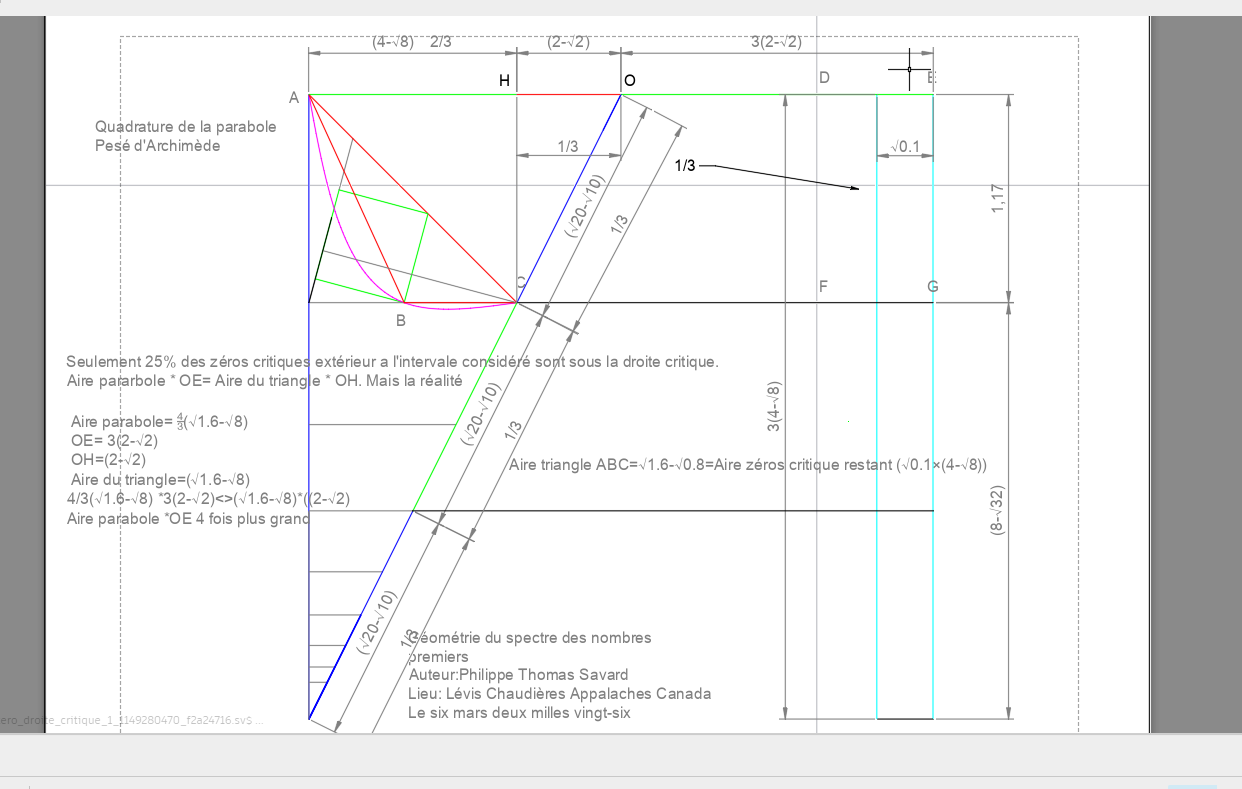
\includegraphics[width=0.85\textwidth]{quadrature_parabole_zero_critique.png}
    \caption{Quadrature de la parabole — zéros critiques (bloc 1)}
    \label{fig:quadrature_parabole_bloc1}
\end{figure}

\newpage
\section{Tableaux Complets des Deux Suites}

\subsection{Tableau pour le nombre premier 29 (10\textsuperscript{e} nombre premier)}

\begin{center}
\begin{longtable}{|c|c|c|}
\hline
\textbf{Position} & \textbf{Somme 1\textsuperscript{ere} suite} & \textbf{Somme 2\textsuperscript{ieme} suite} \\
\hline
\endfirsthead
\hline
\textbf{Position} & \textbf{Somme 1\textsuperscript{ere} suite} & \textbf{Somme 2\textsuperscript{ieme} suite} \\
\hline
\endhead
1\textsuperscript{ere} & $((1^2)^2 + (2^1)^2)^{1/2}$ & $((1^2)^2 + (2^1)^2)^{1/2}$ \\
\hline
2\textsuperscript{ieme} & $((2^1)^2 + (2^2)^2)^{1/2}$ & $((2^1)^2 + (2^2)^2)^{1/2}$ \\
\hline
3\textsuperscript{ieme} & $((2^2)^2 + (2^3)^2)^{1/2}$ & $((2^2)^2 + (2^3)^2)^{1/2}$ \\
\hline
4\textsuperscript{ieme} & $((2^3)^2 + (2^4)^2)^{1/2}$ & $((2^3)^2 + (2^4)^2)^{1/2}$ \\
\hline
5\textsuperscript{ieme} & $((2^4)^2 + (2^5)^2)^{1/2}$ & $((2^4)^2 + (2^5)^2)^{1/2}$ \\
\hline
6\textsuperscript{ieme} & $((2^5)^2 + (2^6)^2)^{1/2}$ & $((2^6)^2 + (2^7)^2)^{1/2}$ \\
\hline
7\textsuperscript{ieme} & $((2^6)^2 + (2^7)^2)^{1/2}$ & $((2^7)^2 + (2^8)^2)^{1/2}$ \\
\hline
8\textsuperscript{ieme} & $((2^7)^2 + (2^8)^2)^{1/2}$ & $((2^8)^2 + (2^9)^2)^{1/2}$ \\
\hline
9\textsuperscript{ieme} & $((2^8)^2 + (2^9)^2)^{1/2} \times (2^{-1})$ & $((2^9-2^7)^2 + (2^{10}-2^8)^2)^{1/2}$ \\
\hline
10\textsuperscript{ieme} & $((2^9-2^7)^2 + (2^{10}-2^8)^2)^{1/2}$ & $((2^{10}-2^8)^2 + (2^{11}-2^9)^2)^{1/2}$ \\
\hline
\textbf{Somme} & $\sqrt{3452805}$ & $\sqrt{13300805}$ \\
\hline
\end{longtable}
\end{center}

\textbf{Verification du nombre premier :}
\[
\frac{\sqrt{13300805} - \sqrt{2471045}}{\sqrt{5120}} = 29
\]
Toute contribution volontairement soumise par Vous a l'Auteur dans le but
d'etre integree au Travail (incluant le code HOL, le code LaTeX, les
modeles mathematiques ou tout contenu associe) est reputee etre fournie
selon les termes de la presente Licence, sauf indication ecrite contraire
de Votre part. Aucune clause de la presente Licence ne modifie ou ne
remplace les termes d'un accord distinct que Vous auriez conclu avec
l'Auteur concernant ces contributions.

\subsection*{10/9.1 Marques et attribution}

La presente Licence ne Vous accorde aucun droit d'utiliser le nom,
l'identite, les logos, les marques ou les designations de l'Auteur a des
fins promotionnelles ou commerciales. Vous pouvez toutefois mentionner
l'Auteur uniquement pour decrire l'origine du Travail ou pour reproduire
fidelemenent les avis de droits d'auteur.

\subsection*{10/9.2 Absence de garantie}

Sauf exigence contraire de la loi ou accord ecrit, le Travail est fourni
"en l'etat", sans garantie d'aucune sorte, explicite ou implicite,
incluant notamment les garanties de titre, de non-contrefacon, de qualite
marchande ou d'adequation a un usage particulier. Vous etes seul
responsable de determiner l'adequation du Travail a Vos besoins et
d'assumer les risques lies a son utilisation ou a sa redistribution.

\subsection*{10/9.3 Limitation de responsabilite}

En aucun cas, et selon aucune theorie juridique (responsabilite civile,
contractuelle ou autre), l'Auteur ne pourra etre tenu responsable de
dommages directs, indirects, speciaux, accessoires ou consecutifs
resultant de l'utilisation ou de l'impossibilite d'utiliser le Travail,
incluant notamment la perte de donnees, l'interruption d'activite, les
defaillances informatiques ou tout autre prejudice commercial, meme si
l'Auteur a ete informe de la possibilite de tels dommages.

\subsection*{10/9.4 Acceptation de garanties ou responsabilites supplementaires}

Lors de la redistribution du Travail ou d'oeuvres derivees, Vous pouvez
choisir d'offrir des garanties, du support, une indemnisation ou toute
autre forme de responsabilite supplementaire. Toutefois, Vous ne pouvez
agir qu'en Votre nom propre et en Votre seule responsabilite. Vous devez
indemniser et degager l'Auteur de toute responsabilite resultant des
obligations supplementaires que Vous acceptez d'assumer.

Toute garantie ou responsabilite supplementaire que vous choisissez
d'assumer l'est en votre nom propre.



\end{document}